\documentclass[10pt]{beamer}

\ifx\pdfoutput\undefined
% we are running LaTeX, not pdflatex
\usepackage{graphicx}
\else
% we are running pdflatex, so convert .eps files to .pdf
\usepackage{CJKutf8}
\usepackage{graphicx}
\usepackage{epstopdf}
\fi

\input{beihangbeamerstyle/beihangcolor}
\input{beihangbeamerstyle/beihangbeamerstyle}

\title{Neural image compression with scene graphs}
\author{道尔格 (\texttt{ls1906205@buaa.edu.cn})}
\date{Thesis proposal defence, Beihang University, Fri  21 May 2021}


\begin{document}
%----------------------------------------------------------------------
% Title frame
\begin{frame}[plain]
    \maketitle
\end{frame}

%----------------------------------------------------------------------
% Outline frame
% PLEASE RUN pdflatex TWICE 
\begin{frame}
    \frametitle{Outline}
    \tableofcontents
\end{frame}
%%=====================================================================

\section{Introduction}

\begin{frame}
    \frametitle{Introduction}
    \begin{block}{Image compression}
        Image compression is an important task in computer science and engineering.
        Two main approaches:
        \begin{itemize}
            \item Lossy (estimating information). JPEG etc.
            \item Lossless (compressing information). DEFLATE etc.
        \end{itemize}
        Discrete cosine transform (DCT), Huffman coding.
    \end{block}
\end{frame}

\begin{frame}
    \frametitle{JPEG}
    Famous JPEG format, for example, has following steps, and only last three are about compression.

    \begin{enumerate}
        \item Encoding RGB to YCbCr (Chroma subsampling).
        \item Discrete Cosine Transform. Lossy compression.
        \item Run-length encoding. Lossless compression.
        \item Huffman encoding. Lossless compression.
    \end{enumerate}
\end{frame}

\begin{frame}
    \frametitle{Compression}
    \begin{columns}
        \begin{column}{0.5\textwidth}
            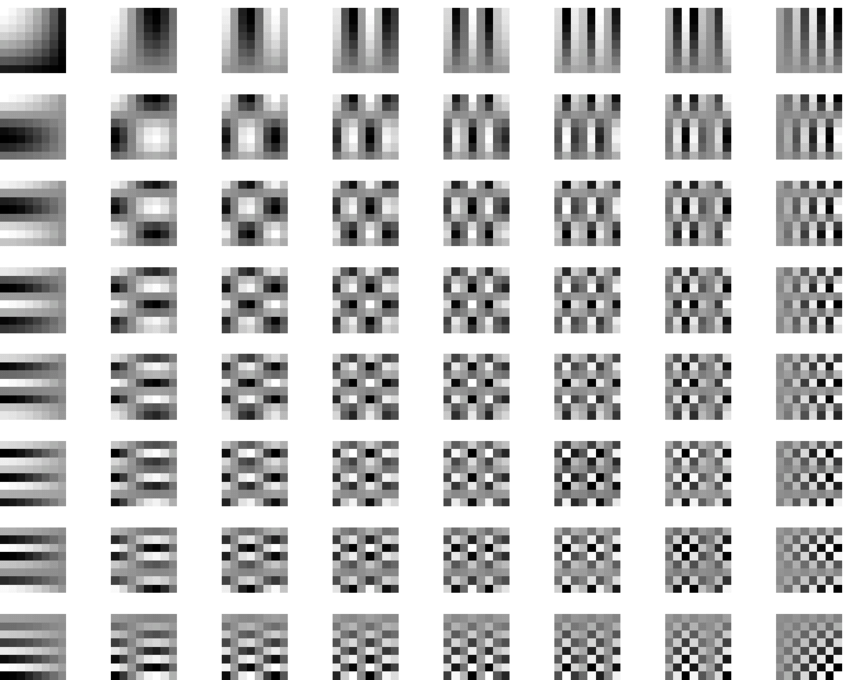
\includegraphics[width=\textwidth]{figure/2d-dct.png}
        \end{column}
        \begin{column}{0.5\textwidth}
            \begin{block}{Image compression}

                It is common to use DCT based methods in image compression. A popular implementation of Fourier transform for discrete functions is Discrete Cosine Transform.

                However this is not the only one approach. Instead of using a predefined polynomial to encode an image, it is possible to use neural networks to pack and unpack information.

            \end{block}
        \end{column}
    \end{columns}
\end{frame}

\begin{frame}
    \frametitle{Neural compression}
    There were several approaches to apply neural networks architecture in image compression. Take an autoencoder architecture as an example:
    \begin{block}{Autoencoder for compression}
        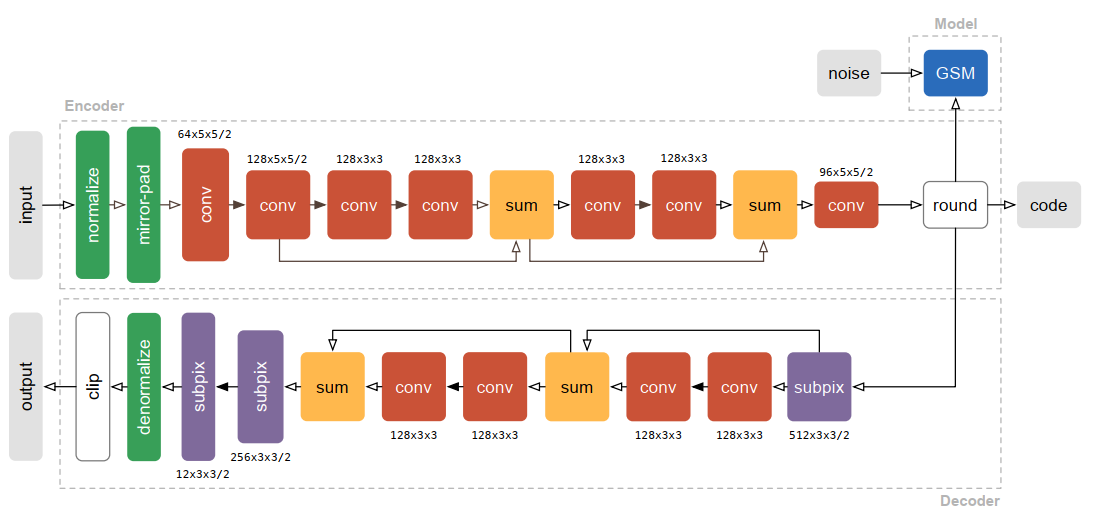
\includegraphics[width=\textwidth]{figure/neural-compression.png}
    \end{block}
\end{frame}


\begin{frame}
    \frametitle{Image and sene gaph}
    \begin{columns}
        \begin{column}{0.5\textwidth}
            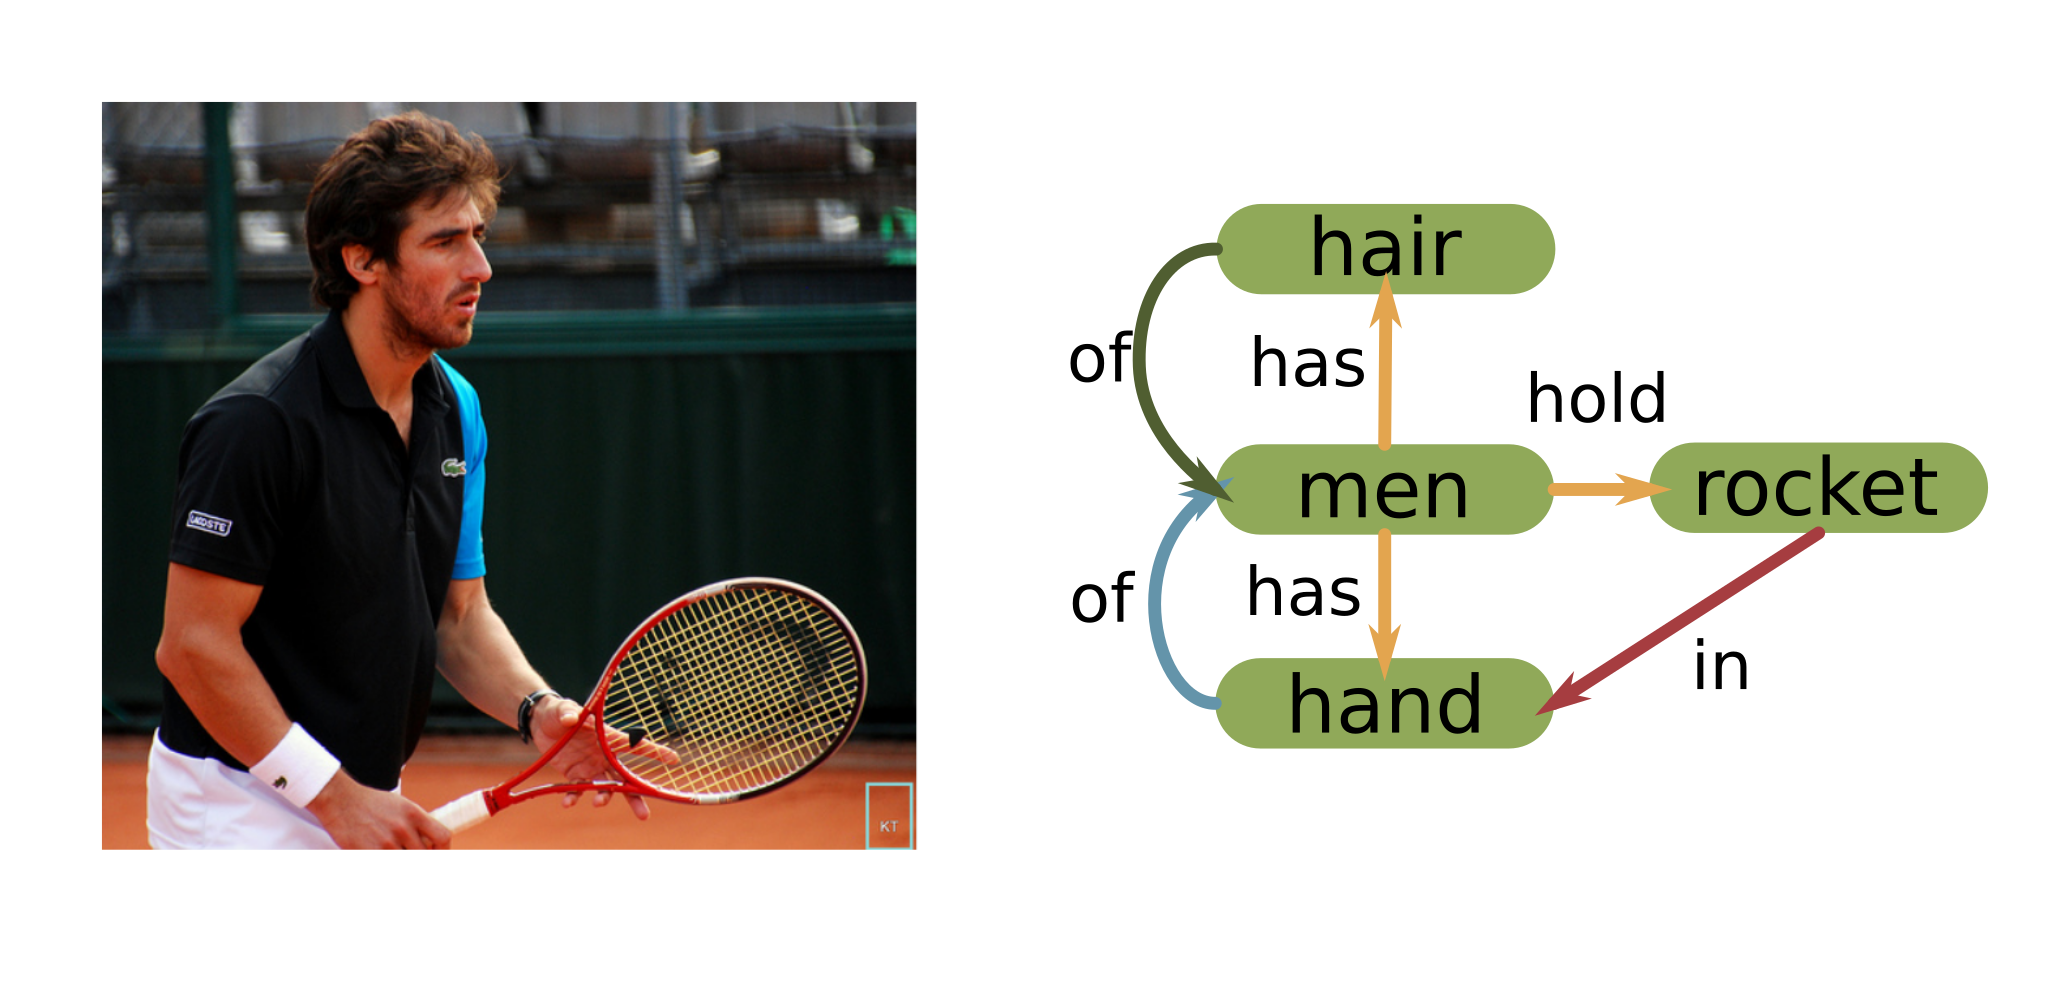
\includegraphics[width=\textwidth]{figure/image-and-scene-graph.png}
        \end{column}
        \begin{column}{0.5\textwidth}
            How do we memorize image or visual scene in our life. We do not operate in terms of pixels or object coordinates. More likely we use something like scheme, which describes the most important parts of an image.
            There are already algorithms capable to extract Scene Graphs form image. There are some approaches to generate an image from scene graphs. We can combine those two.
        \end{column}
    \end{columns}
\end{frame}

\begin{frame}
    \frametitle{Niches}

    Potential application niches:

    \begin{enumerate}
        \item Limited space on machine with high computational power.
        \item Huge images needed to be transmitted through a network with limited speed.
    \end{enumerate}

    TODO : verbally describe limitations
\end{frame}

\section{Methodology}
\begin{frame}
    \frametitle{Methodology}

    A general approach is to use two models: one model will be used to generate intermediate representation, another one will be used to restore an original image from its representation.

\end{frame}

\begin{frame}
    \frametitle{Image scene graph}

    \begin{columns}
        \begin{column}{0.5\textwidth}
            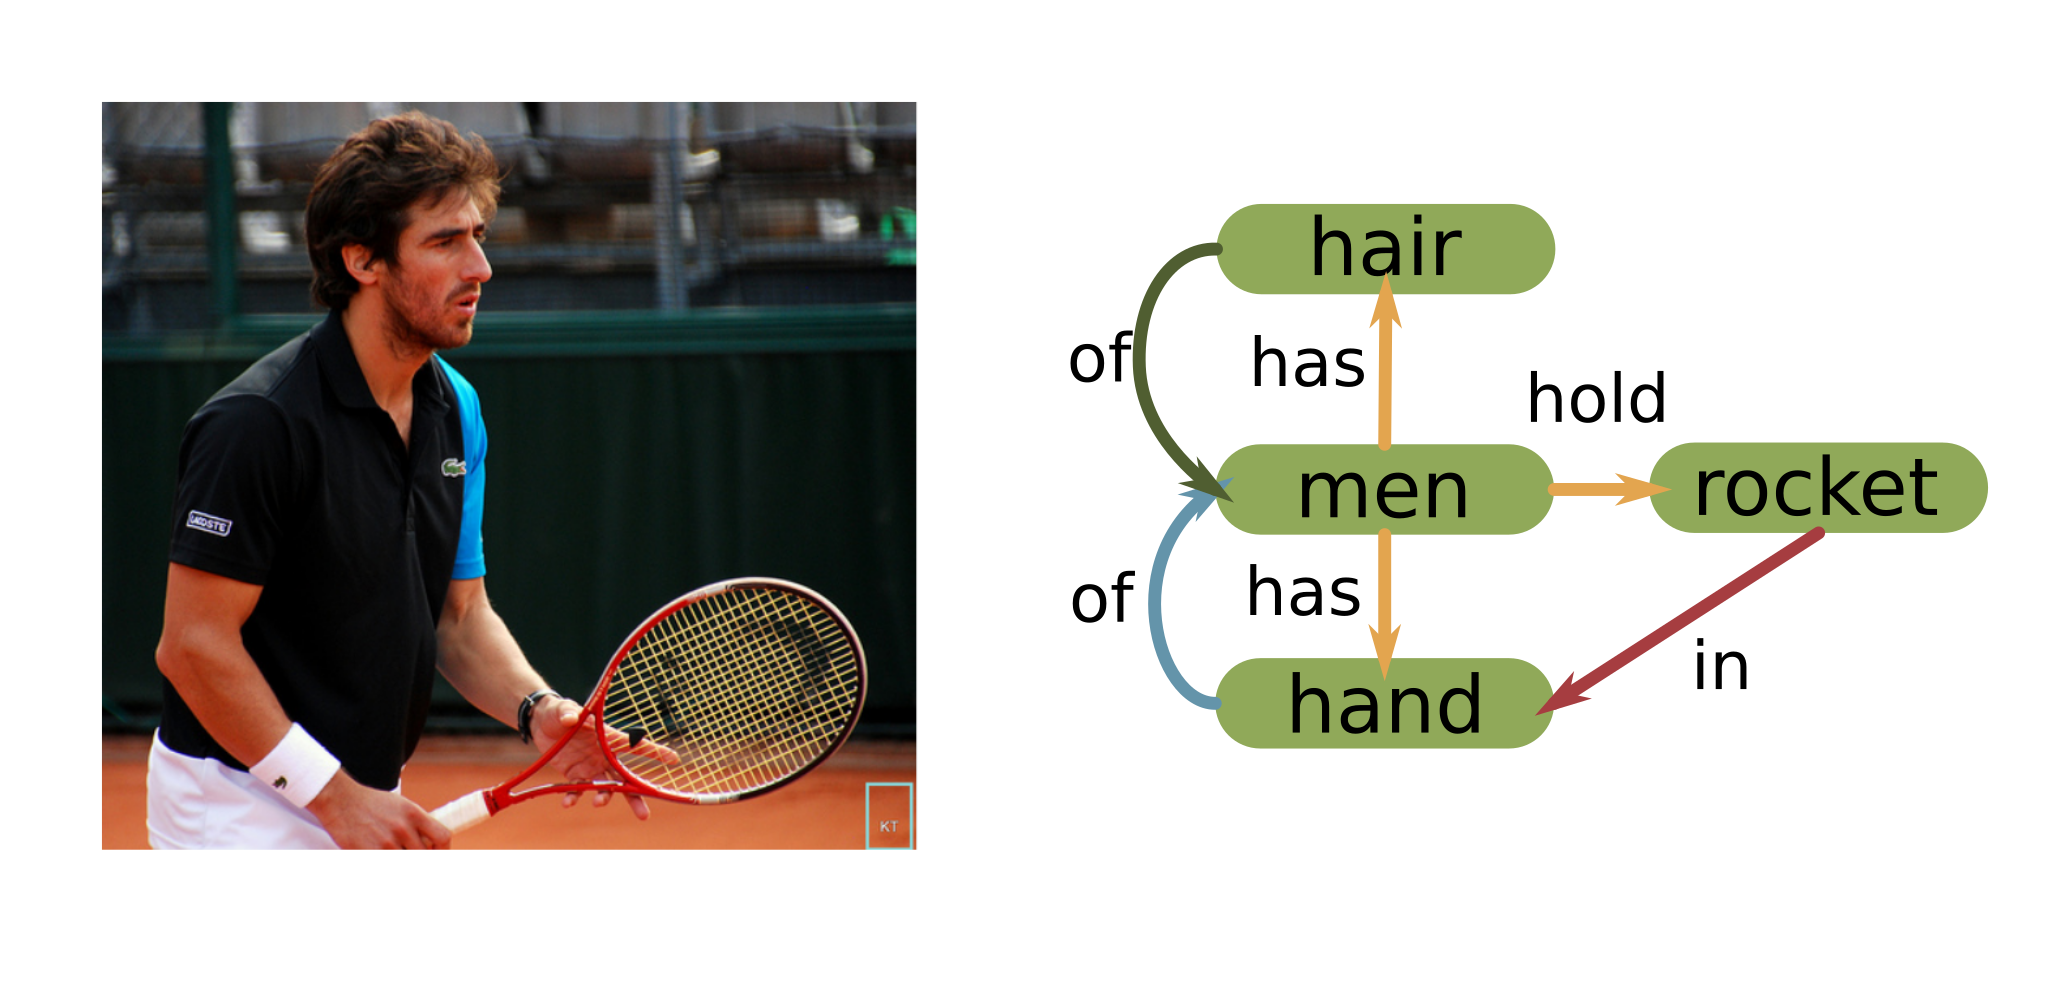
\includegraphics[width=\textwidth]{figure/image-and-scene-graph.png}
        \end{column}

        \begin{column}{0.5\textwidth}
            On the left we can see an image scene graph.
        \end{column}
    \end{columns}
\end{frame}

\begin{frame}
    \frametitle{General pipeline}

    First scene graph and convolution features are obtained. Then this can be treated as a compressed representation of initial image. It can be sent through network or being stored on machine. When the original image is needed we can feed this representation to generative model to obtain initial image.

    \begin{block}{General pipeline}
        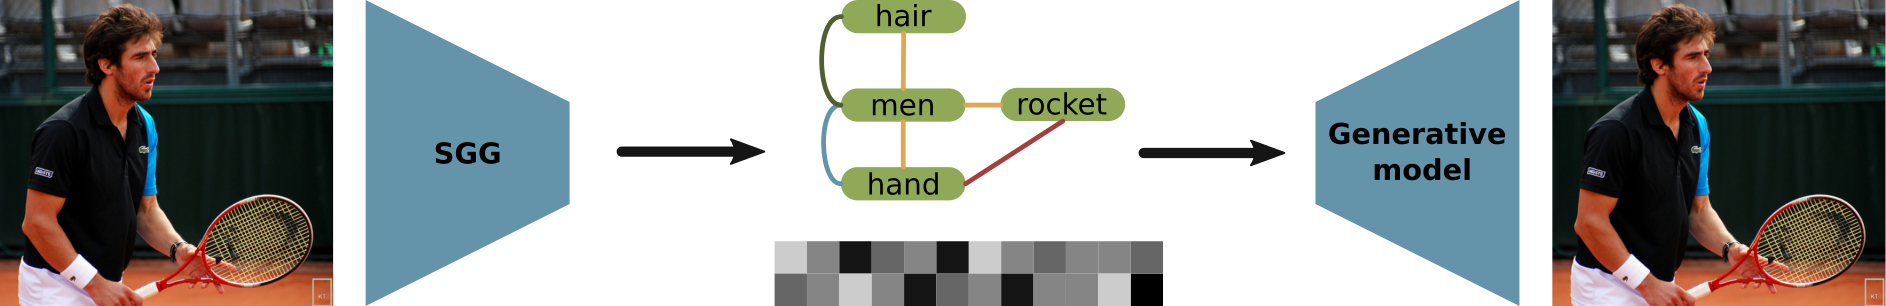
\includegraphics[width=\textwidth]{figure/application-general-pipeline.png}
    \end{block}
\end{frame}

\begin{frame}
    \frametitle{Scene graph example}

    \textbf{Scene graph generation general view.} The left part is original image, the middle part is image with detected objects and the right part is scene graph that can be obtained from such image.

    \begin{block}{}
        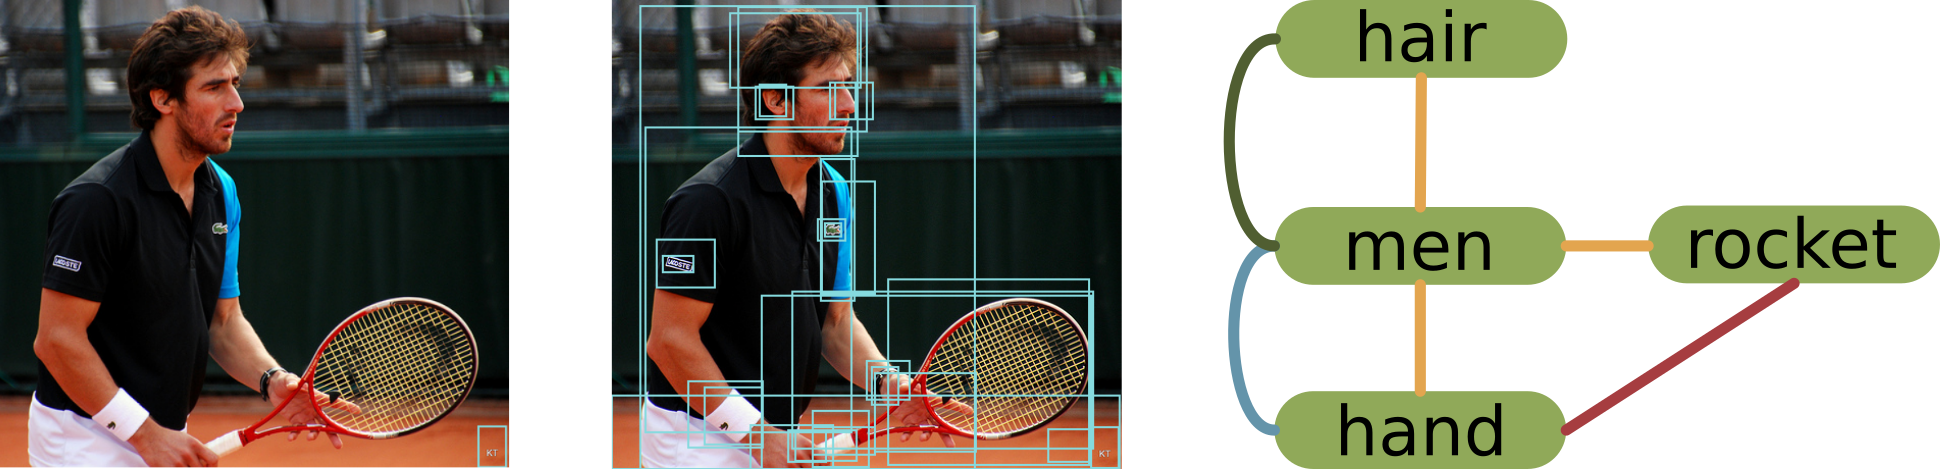
\includegraphics[width=\textwidth]{figure/scene-graph-example.png}
    \end{block}
\end{frame}

\begin{frame}
    \frametitle{Scene graph generation}

    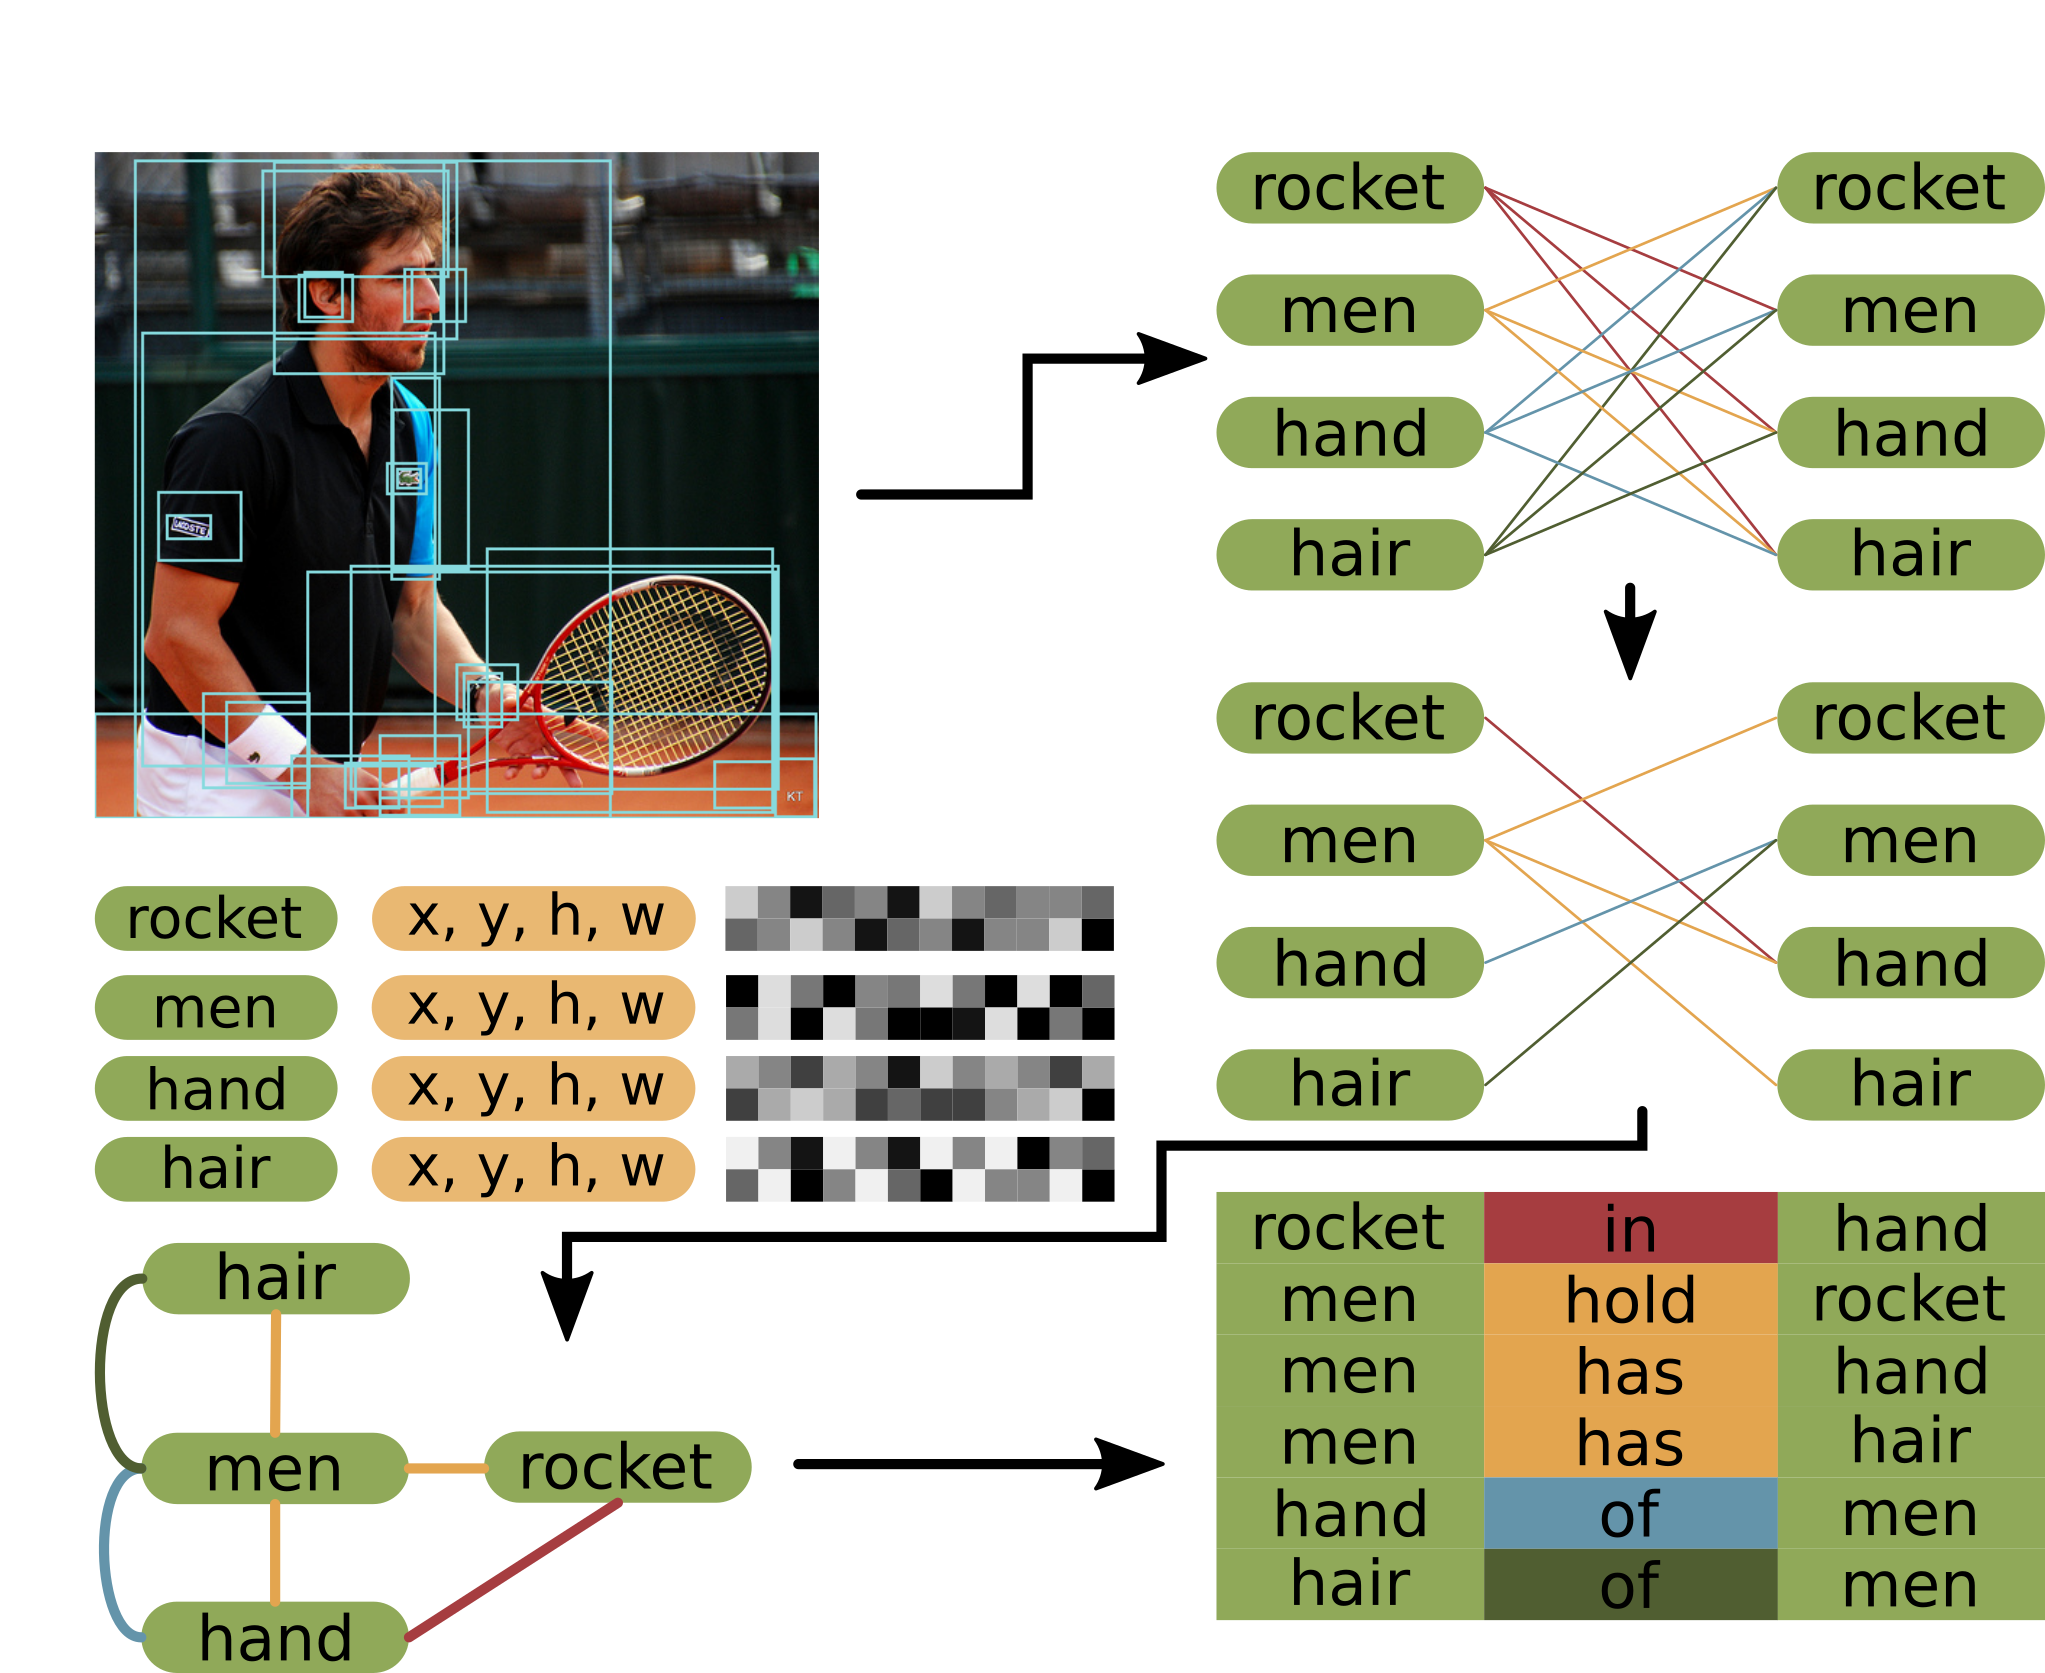
\includegraphics[height=150pt]{figure/sgg-pipeline.png}

\end{frame}

\begin{frame}
    \frametitle{Image generation pipeline}

    General pipeline to generate an image from an arbitrary scene graph. We use additional information from compression step to obtain bounding boxes and convolutional features to 
    \begin{block}{Image generation}
        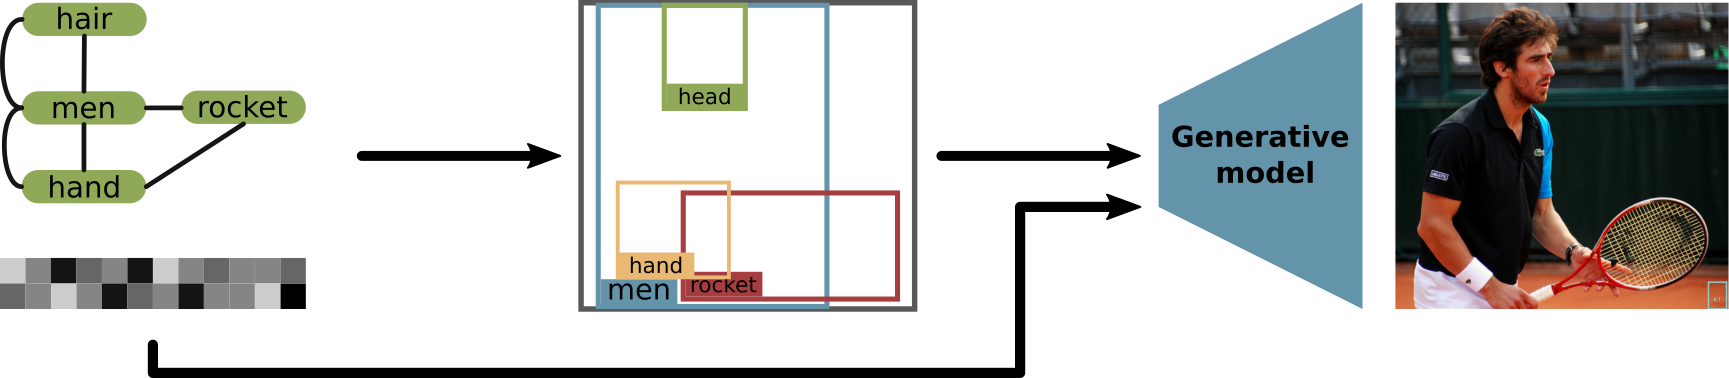
\includegraphics[width=\textwidth]{figure/image-generation-from-sg.png}
    \end{block}
\end{frame}

\section{Data}
\begin{frame}
    \frametitle{Data}

    Visual Genome dataset consists of more than 100,000 images labeled with scene graphs.

    Dataset structure:
    \begin{enumerate}
        \item Region descriptions. Human labeled important regions of an image, each description phrase is 1 to 16 words long.
        \item Objects. Objects labeled and canonicalized to a synset ID in WordNet.
        \item Attributes. Both images and objects have attributes. They are also canonicalized to WordNet.
        \item Relationships. Connects a pair of objects. Relationships are directed.
        \item Region graphs. A graph of a region of an image. These could be more than one region graph on one image.
        \item Scene graphs. A composition of region graph of an image. One image has exactly one scene graph.
        \item Question-answer pairs. There are both region-based and freeform QA pairs.
    \end{enumerate}
\end{frame}

\section{Planning and arrangement}
\begin{frame}
    \frametitle{Future planing}

    \begin{table}
        \centering
        \begin{tabular}{p{3cm}|p{5cm}|p{2cm}}
            \hline
            Task                                            & Description                                                                                                                                & Deadline    \\
            \hline
            Build a model prototype                         & Build a first version of a model that is capable to compress and restore images, it will include building and training encoder and decoder & September 1 \\
            \hline
            Improve model prototype                         & Adjust parameters, decide on additional convolutional features size                                                                        & December 1  \\
            \hline
            Pack model and make it accessible for engineers & Choose an approach to pack model, implement clean and reusable library                                                                     & March 1     \\
            \hline
            Write the final thesis up                       & Summarize research in the final thesis                                                                                                     & June 1      \\
            \hline
        \end{tabular}
    \end{table}

\end{frame}

\end{document}
